\documentclass{ctexbeamer}
%\tiny\scriptsize\footnotesize\small\normalsize\large\Large\LARGE \huge\Huge
\useoutertheme{metropolis}
\useinnertheme{metropolis}
%\usefonttheme{metropolis}
\usecolortheme{crane}
\setbeamertemplate{frame numbering}[fraction]		% 当前页/总页数
%\setbeamertemplate{headline}{}						% 不显示最上的导航栏
%\setbeamertemplate{navigation symbols}{}			% 不显示右下的导航图标
\setbeamercovered{transparent=15}					% pause 透明度

%\usefonttheme{professionalfonts} % using non standard fonts for beamer
\usefonttheme{serif} % default family is serif

\setbeamerfont{footnote mark}{size=\scriptsize}		% 脚注符号大小
\setbeamerfont{footnote}{size=\footnotesize}		% 脚注大小
\setbeamerfont{title}{shape=\itshape,family=\rmfamily}	% 总标题字体
\setbeamerfont{frametitle}{size=\large}					% 页标题字体

\newcommand{\Sub}{$>>>$}

\usepackage{tikz}
\usetikzlibrary{arrows,patterns,plotmarks,shapes,snakes,er,3d,automata,backgrounds,topaths,trees,petri,mindmap}

\XeTeXlinebreaklocale "zh"							% 表示用中文的断行
\XeTeXlinebreakskip = 0pt plus 1pt					% 多一点调整的空间


\usefonttheme[onlylarge]{structuresmallcapsserif}
\usefonttheme[onlysmall]{structurebold}
%\setbeamercolor{title}{fg=red!80!black,bg=red!20!white}

\def\hilite<#1>{%
\temporal<#1>{\color{gray}}{\color{blue}}%
{\color{blue!45}}}
\renewcommand{\raggedright}{\leftskip=0pt \rightskip=0pt plus 0cm}
\raggedright

\usepackage{pstricks,pst-tree,pst-node,pst-text}
\usepackage{multicol}
\usepackage{amsmath}
\usepackage{listings}
\usepackage{tabularx}

\definecolor{commentcolor}{RGB}{85,139,78}
\definecolor{stringcolor}{RGB}{206,145,108}
\definecolor{keywordcolor}{RGB}{34,34,250}
\definecolor{backcolor}{RGB}{220,220,220}


% 代码环境
\lstset{
%backgroundcolor = \color{gray!10},
numbers=left, 									% 左侧行号,删除本行则无行号
numbersep=8pt,                   				% 行号与代码的间距
%flexiblecolumns=true,             				% 加上后tabsize不准确
numberstyle=\scriptsize, 	
stepnumber=1,                   				% 行号出现的间隔数,是1的话每行都标注行号
basicstyle=\linespread{1}\small\ttfamily, 		% 代码基本设置,行间距,字体大小
commentstyle=\color{commentcolor},  			% 注释
keywordstyle=\bfseries\color{keywordcolor},  	% 关键词加粗
stringstyle=\color{red},    					% 字符串
%escapeinside=&&,								% 逃逸字符,基本不用
extendedchars=true,           					% lets you use non-ASCII characters; for 8-bits encodings only, does not work with UTF-8
frame=shadowbox, % trBL, 
rulesepcolor= \color{red!20!green!20!blue!20},	% 阴影浅灰色
%xleftmargin=2em,								
%xrightmargin=2em,
%aboveskip=1em,
tabsize=4,										% tab的空格数
breaklines=true,  							 	% 自动换行,建议不要写太长的行
%title=\lstname	% show the filename of files included with \lstinputlisting; also try caption instead of title
}

%\setmonofont{Courier New}

\setbeamertemplate{blocks}[rounded][shadow=true]
\setbeamercolor{block body alerted}{bg=alerted text.fg!10}
\setbeamercolor{block title alerted}{bg=alerted text.fg!20, fg=red}
\setbeamercolor{block body}{bg=structure!10}
\setbeamercolor{block title}{bg=structure!20, fg=red}
\setbeamercolor{block body example}{bg=green!10}
\setbeamercolor{block title example}{bg=green!20}

\usepackage{colortbl}

%修改比例16:9
\usepackage[orientation=landscape,size=custom,width=16,height=9,scale=0.36,debug]{beamerposter}

%伪代码设置
\usepackage[lined]{algorithm} 
\usepackage{amsthm}
\usepackage[noend]{algpseudocode}

\algnewcommand{\algorithmicand}{\textbf{ and }}
\algnewcommand{\algorithmicor}{\textbf{ or }}
\algnewcommand{\Or}{\algorithmicor}
\algnewcommand{\AND}{\algorithmicand}
\algnewcommand{\Break}{\textbf{break} }
\makeatletter
\def\BState{\State\hskip-\ALG@thistlm}
\makeatother


\begin{document}
\graphicspath{{assets/}}

\title{Title \ Title Title \\ Title Title}
\author{author\\ \texttt{xxxxxx@xxx.com}}
\date{ \today}

\frame[plain]\titlepage

\begin{frame}[containsverbatim]
\frametitle{Block \& Image\footnote{footnote}}
	\begin{block}{Definition}
		A vertex cover of a graph is a set of vertices such that each edge of the graph is incident to at least one vertex of the set.
	\end{block}

	\begin{figure}[h!]
		\centering
		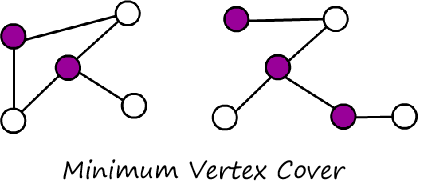
\includegraphics[scale=0.6]{example.png}	% 注意图片路径
	\end{figure}
\end{frame}


\begin{frame}[containsverbatim]{Code Example}
	\begin{columns}[c]
		\column{0.5\textwidth}
		\begin{lstlisting}[language=C++,aboveskip=0pt,basicstyle=\linespread{1.1}\small\ttfamily]
bool dfs(int x) {
	for (auto &y:e[x])
	if (!used[y]) {
		used[y] = true;
		if (link[y] == -1 || dfs(link[y])) {
			link[y] = x;
			return true;
		}
	}
	return false;
}
\end{lstlisting}
		\column{0.48\textwidth}
		\begin{lstlisting}[language=C++,aboveskip=0pt,basicstyle=\linespread{1.1}\small\ttfamily]
int hungary() {
	int res = 0;
	memset(link, -1, sizeof(link));
	for (int i = 1; i <= n; ++i) {
		memset(used, false, sizeof(used));
		if (dfs(i)) ++res;
	}
	return res;
}
\end{lstlisting}
	\end{columns}
\end{frame}


\begin{frame}[containsverbatim]\frametitle{Pseudocode 伪代码}
	\begin{itemize}
		\item numerical analysis, computational geometry...
		\item time complexity $O(\log{((R-L)/\epsilon)})$
	\end{itemize}

	\begin{algorithm}[H]
		\label{BinarySearch}
		\begin{algorithmic}[1]
			\Procedure{BinarySearchOnRealNumbers}{$L,R$}
			\While {$R-L>\epsilon$}
			\State $mid \gets (L+R)/2$
			\If{\Call{lessThanAns}{$mid$}}
			\State $L \gets mid$
			\Else
			\State $R \gets mid$
			\EndIf
			\EndWhile
			\Return $L$
			\EndProcedure
		\end{algorithmic}
	\end{algorithm}
\end{frame}


\begin{frame}[t, fragile]\frametitle{Pause}
	\begin{itemize}
		\item 测试一下{\red pause}语句的功能
	\end{itemize}

	\pause
	\begin{block}{任务}
		统计及格学生的平均成绩(不计不及格的学生和分数)
	\end{block}

	\pause
	\begin{columns}[t]

		\column{0.45\textwidth}
		\begin{lstlisting}[language=Python]
scores = [76, 83, 89, 45, 67, 89, 85, 77]
sum_, count = 0, 0
for score in scores:
    if score < 60:
        continue
    sum_ += score
    count += 1
print('平均成绩为:', sum_/count)
\end{lstlisting}

		\column{0.45\textwidth}
		\pause
		\begin{lstlisting}[language=Python]
scores = [76, 83, 89, 45, 67, 89, 85, 77]
sum_, count = 0, 0
for score in scores:
    if score >= 60:
        sum_ += score
        count += 1
print('平均成绩为:', sum_/count)
\end{lstlisting}
	\end{columns}

\end{frame}

\begin{frame}{TIKZ}

	\vspace{10pt}

	\begin{block}{任务}
		将正则表达式$(a\mid b)*a(a\mid b\mid \epsilon)$转化成一个DFA并最小化
	\end{block}

	\begin{columns}[t] % 对齐方式 top aligning
		\column{0.45\textwidth}
		先构造出NFA,之后使用\textbf{子集构造法}转DFA
		\begin{figure}[ht]
			\centering
			\begin{tikzpicture}[->,>=stealth',shorten >=1pt,auto,node distance=2cm,
					thick,base node/.style={circle,draw,minimum size=16pt}, real node/.style={double,circle,draw,minimum size=35pt}]
				\node[initial,initial text={},state] (A) {$A$};
				\node[accepting, state](B)[above right of=A]{$B$};
				\node[state](C)[below right of=A]{$C$};
				\node[accepting, state](D)[right of=B]{$D$};
				\node[accepting, state](E)[right of=C]{$E$};

				\path[]
				(A) edge [above]node {$a$} (B)
				(A) edge [below]node {$b$} (C)
				(B) edge [above]node {$a$} (D)
				(B) edge [bend left,below]node {$b$} (E)
				(C) edge [loop below]node {$b$} (C)
				(C) edge [left]node {$a$} (B)
				(D) edge [loop above]node {$a$} (D)
				(D) edge [right]node {$b$} (E)
				(E) edge [bend left , above]node {$a$} (B)
				(E) edge [below]node {$b$} (C);
			\end{tikzpicture}
		\end{figure}

		\column{0.45\textwidth}
		\textbf{最小化} $1:\{A,C\},2:\{B,D\},3:\{E\}$
		\begin{figure}[ht]
			\centering
			\begin{tikzpicture}[->,>=stealth',shorten >=1pt,auto,node distance=2cm,
					thick,base node/.style={circle,draw,minimum size=16pt}, real node/.style={double,circle,draw,minimum size=35pt}]


				\node[initial,initial text={},state] (1) {$1$};
				\node[accepting, state](2)[above right of=1]{$2$};
				\node[accepting, state](3)[below right of=2]{$3$};

				\path[]
				(1) edge [loop below]node {$b$} (1)
				(1) edge [above]node {$a$} (2)
				(2) edge [loop above]node {$a$} (2)
				(2) edge [bend left,below]node {$b$} (3)
				(3) edge [below]node {$b$} (1)
				(3) edge [bend left,below]node {$a$} (2);
			\end{tikzpicture}
		\end{figure}

	\end{columns}
\end{frame}

\begin{frame}{Math Formula}
	\fontsize{12pt}{14pt}\selectfont % size 12pt, vskip=10pt
	本页的字体大小为12pt,vskip为14pt
	\begin{itemize}
		\item 欧拉公式:

		      $$e^{i\pi}+1=0$$
		\item 拉格朗日插值:

		      $$A(x)=\sum_{k=0}^{n-1}y_k\frac{\prod_{j\ne k}(x-x_j)}{\prod_{j\ne k}(x_k-x_j)}$$

	\end{itemize}

\end{frame}


\begin{frame}{Table}
	\begin{block}
		{
			\centering
			\begin{tabularx}{\dimexpr\textwidth-2\tabcolsep}{@{}p{0.2\textwidth}@{}p{0.2\textwidth}@{}p{0.2\textwidth}@{}p{0.133\textwidth}@{}p{0.133\textwidth}@{}p{0.133\textwidth}}
				Algorithm & Time (worst) & Time (avg.) & Space & Stable & In-place
			\end{tabularx}
		}%
		\centering
		\begin{tabularx}{\dimexpr\textwidth-2\tabcolsep}{@{}p{0.2\textwidth}@{}p{0.2\textwidth}@{}p{0.2\textwidth}@{}p{0.133\textwidth}@{}p{0.133\textwidth}@{}p{0.133\textwidth}}

			insertion sort & $\Theta(n^2)$      & $\Theta(n^2)$      & $O(1)$               & yes & yes \\
			merge sort     & $\Theta(n\log{n})$ & $\Theta(n\log{n})$ & $O(N)$               & yes & no  \\
			heapsort       & $O(n\log{n})$      & $O(n\log{n})$      & $O(1)$               & no  & yes \\
			quick sort     & $\Theta(n^2)$      & $\Theta(n\log{n})$ & $O(N)$  $O(\log{N})$ & no  & yes \\
			counting sort  & $\Theta(k+n)$      & $\Theta(k+n)$      & $O(k)$               & yes & no  \\
			radix sort     & $\Theta(d(k+n))$   & $\Theta(d(k+n))$   & $O(k+n)$             & -   & no  \\
			bucket sort    & $\Theta(n^2)$      & $\Theta(n)$        & $O(n) $              & yes & no
		\end{tabularx}%
	\end{block}%
\end{frame}

\begin{frame}{Other Tables}

	%\resizebox{10cm}{!}
	%{
	\begin{tabular}{ccccccc}
		\hline
		i & 0  & 1  & 2 & 3  & 4 & 5  \\
		\hline
		s & \$ & \# & a & \# & a & \# \\
		\hline
	\end{tabular}
	%}

	\begin{table}
		\caption{A realistic table I have built}
		\label{tab:table}
		\begin{tabular}{|c||ccc|}
			\hline \hline
			Small col     & \multicolumn{3}{|c|}{Big col}                \\
			\hline
			Grouped items & \multicolumn{3}{|c|}{Item 1}                 \\
			\cline{2-4}
			              & \multicolumn{3}{|c|}{Item 2}                 \\
			\hline
			Usual row     & Spam                          & Bacon & Eggs \\
			\hline\hline
		\end{tabular}
	\end{table}

\end{frame}
\end{document}